\chapter{Sistema}

\section{Guía de Uso}

	\subsection{Introducción}
		
		Esta sección pretende mostrar una vista general de la aplicación y sus opciones. A lo largo de ellan se explicarán todos los módulos del programa con los que el usuario tiene contacto y detallará la función de determinados mecanismos.\\
		
		\begin{figure}[htbp]
		\centering
		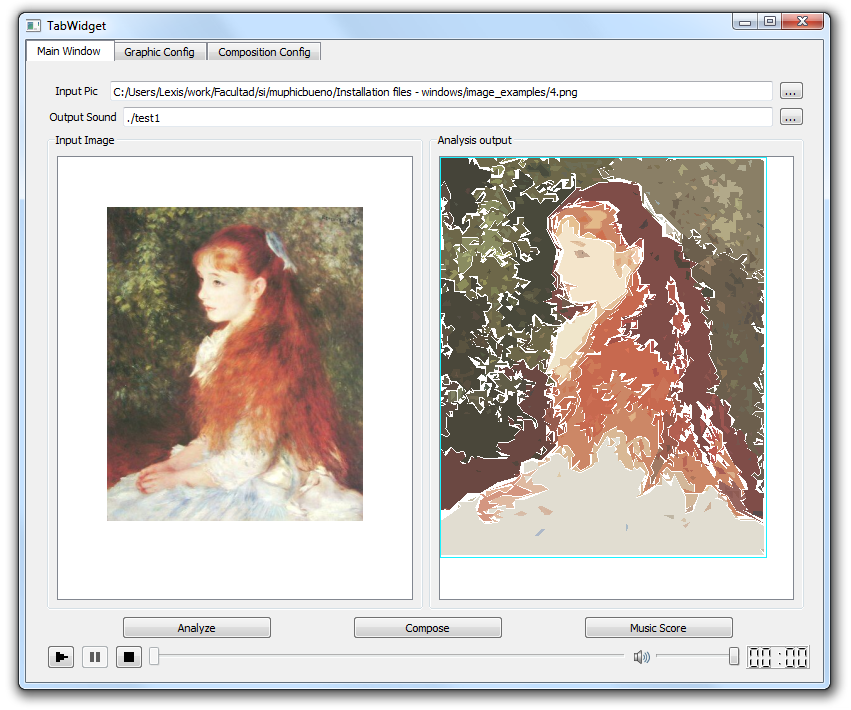
\includegraphics[scale=0.57]{graphics/interfazoverview.png}
		\caption{Vista general de la aplicación}
		\label{fig:interfazoverview}
		\end{figure}
		
		Como vemos en la Figura~\ref{fig:interfazoverview}, la aplicación dispone de 3 pestañas: Main Window, Graphic Config y Composition Config. La primera dispone de toda la funcionalidad necesaria para lanzar la aplicación, mientras que las otras 2 aportan opciones para configurar el comportamiento del análisis y la composición.\\
		
		De forma general, todo usuario, experto o inexperto, se puede valer de la primera pestaña para usar la composición. Sin embargo, un usuario avanzado con conocimientos musicales y de qué tipos de análisis gráficos se realizan puede navegar por las pestañas restantes para configurar el completo proceso mediante los parámetros ofrecidos.
		
		Se procede por tanto a explicar cada pestaña una por una.

		\subsubsection{Ventana principal}
		
		Se encarga de la interacción directa con el usuario; muestra los resultados obtenidos y permite lanzar los distintos componentes de la aplicación. 
		\\Esta compuesta por los siguientes elementos tal y como se puede ver en la Figura~\ref{fig:interfaz}:\\
		
		
		\begin{figure}[htbp]
		\centering
		\hspace*{-0.9in}
		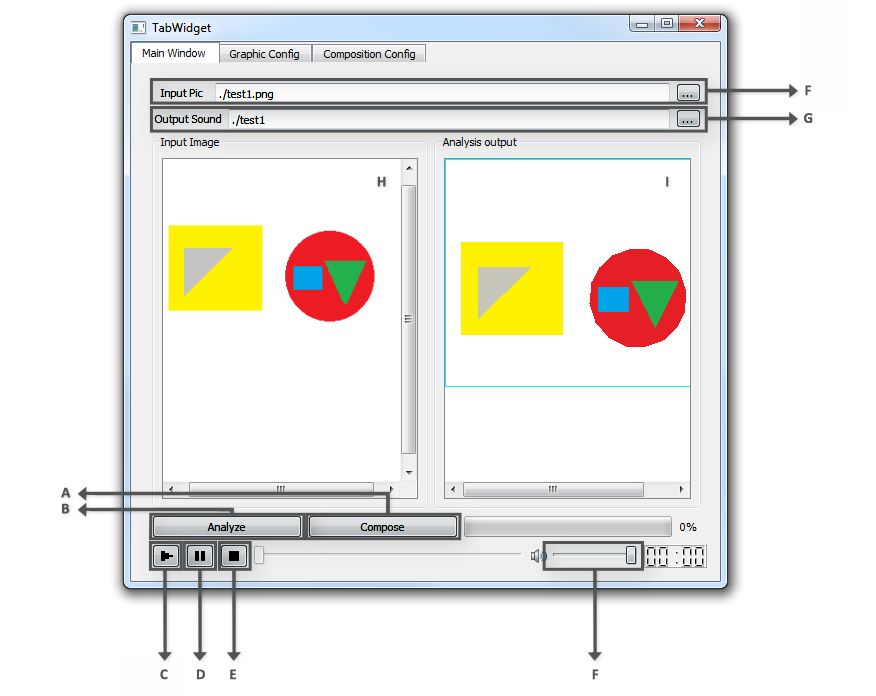
\includegraphics[scale=0.57]{graphics/interfaz.png}
		\caption{Vista general de la pestaña principal de la aplicación}
		\label{fig:interfaz}
		\end{figure}
		
		\noindent\textit{Carga de imagen de entrada [7]:}  Mediante esta opción el usuario puede elegir la dirección desde donde se cargará la imagen de entrada que se usará en el análisis. Para elegir la dirección podrá insertar el texto a mano o utilizar el botón para usar el explorador del sistema operativo correspondiente.\\
		
		\noindent\textit{Selección del archivo de audio de salida [8]:}  Mediante esta opción el usuario puede la dirección dodne se guardará el archivo de salida. Para elegir la dirección podrá insertar el texto a mano o utilizar el botón para usar el explorador del sistema operativo correspondiente.\\
		
		\noindent\textit{Input Image [A]:} En este panel se muestra la imagen elegida para el análisis.\\
		
		\noindent\textit{Analysis output [B]:} En este panel se muestra el resultado del último análisis realizado pulsando el botón "Analyze".\\
		
		\noindent\textit{Botón Analyze [2]:} Tal y como su nombre indica, Analyze, realiza el analisis de la imagen pasada como parámetro de entrada lanzando a ejecución el programa Phic, uno de los módulos de la aplicación. Tras analizarse, el resultado podrá observarse en el \textit{[B]}.\\
		
		\noindent\textit{Botón Compose [1]:} Realiza la composición musical a partir de los datos analizados, para ello lanza a ejecución el programa Mu, otro de los módulos de la aplicación. Una vez compuesta la pieza musical, se podrá escuchar mediante los controles de control de sonido.\\
		
		\noindent\textit{Botón de Inicio de Reproducción [3]:} Permite al usuario iniciar la reproducción de la pieza musical compuesta por el módulo Mu.\\
		
		\noindent\textit{Botón de Pausa de Reproducción [4]:} Pausa la pieza musical en reproducción.\\
		
		\noindent\textit{Botón de Detención de Reproducción [5]:} Detiene la reproducción completamente.\\
		
		\noindent\textit{Barra de sonido [6]:} Modifica el volumen de la reproducción en curso.

		
		\subsubsection{Configuración gráfica}
		
		En esta pestaña se encuentran todas las opciones relacionadas con el análisis de la imagen. En ella se podrán configurar opciones que hagan que el proceso de análisis varíe en velocidad, precisión o estilo.\\
		
		De entre los parámetros de configuración, existen los llamados ``generales'', que siempre aparecen visibles al usuario, y los ``específicos'', que complementan a los generales y sólo aparecen cuando el contexto lo especifica. En la Figura~\ref{fig:interfazgraphic} podemos ver detalladamente los parámetros generales.\\
		
		\begin{figure}[htbp]
		\centering
		\hspace*{-0.9in}
		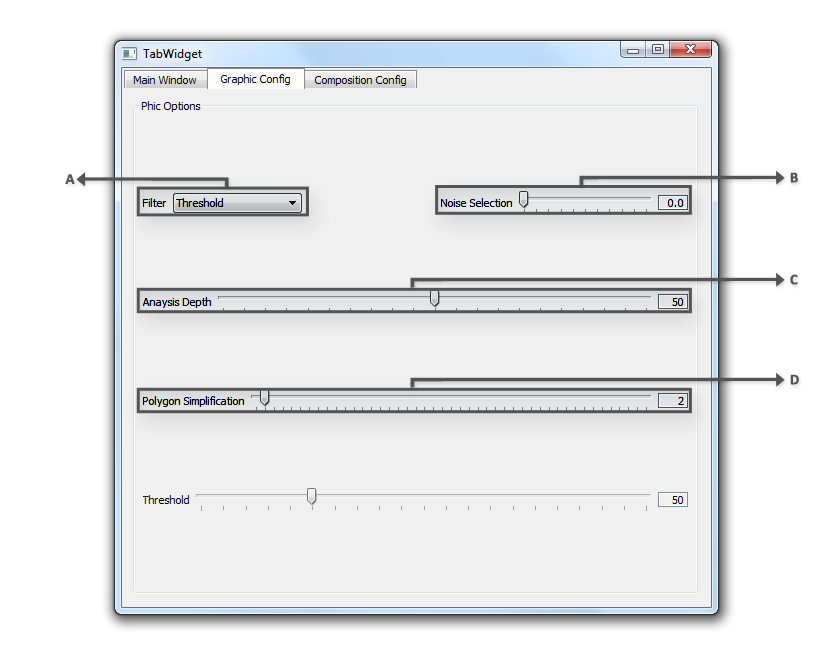
\includegraphics[scale=0.57]{graphics/interfazgraphic.png}
		\caption{Vista general de la pestaña de configuración gráfica}
		\label{fig:interfazgraphic}
		\end{figure}
		
		\noindent\textit{Tipo de filtrado de imagen [1]:} Distintos filtros en la imagen producirán diferentes formas de entender las formas que hay en ellas. De forma un poco más precisa, pero sin llegar a entrar en detalles técnicos, los filtros se encargan de transformar la imagen original a un mapa de bits en blanco y negro, que posteriormente se analizará para detectar polígonos en él. Un buen filtro diferenciará las deseadas superficies de color como manchas blancas independientes.\\
		
		\noindent\textit{Selección de ruido [2]:} Mediante esta barra el usuario puede elegir el tamaño mínimo de las formas por debajo del cual no se considerarán relevantes en el análisis. El valor representa un porcentaje respecto al area total de la imagen, de forma que un valor $n$ de Selección de Ruido determina que todas las formas con area menor a un $n$\% del area total de la imagen se considerarán ruido y no serán estudiadas.\\
		
		\noindent\textit{Profundidad del análisis [3]:} Permite variar el nivel de detalle con el que se realizará el análisis. Un valor de profundidad grande hará que el análisis se realice con gran parte los recursos que permite el programa (a costa de mayor lentitud en el análisis), mientras que un valores pequeños aumentarán la velocidad del proceso a costa de perder precisión a la hora de detectar formas de color.\\
		
		\noindent\textit{Simplificación de polígonos [4]:} Una vez detectadas las formas de color, es necesario aproximarlas a una lista de vértices para reducir el peso de la información sin modificar la carga de la misma. El nivel de fidelidad en la transformación de formas a polígonos se establece con este parámetro: un valor alto determina una gran fidelidad a costa de mayor tiempo de análisis, y viceversa.\\
		
		\noindent\textit{Botón Analyze [2]:} Tal y como su nombre indica, Analyze, realiza el analisis de la imagen pasada como parámetro de entrada lanzando a ejecución el programa Phic, uno de los módulos de la aplicación. Tras analizarse, el resultado podrá observarse en el \textit{[B]}.\\


		Los parámetros ``especícos'' dependen única y exclusivamente del tipo de filtro seleccionado [1], ya que cada tipo de filtro introduce nuevas opciones que configurar. \\
		
		
		Todo filtro en la aplicación que nos ocupa, como ya se comentó anteriormente, realizan la misma función: detectar formas y expresarlas como superficies blancas. A continuación se explica de forma general el funcionamiento de cada filtro y sus parámetros ``específicos''.\\
		
		
		\todo{HACER REFERENCIA A CADA ALGORTIMO QUE NO SEA NUESTRO (TODO MENOS HUE SELECTIONS Y MULTIPLE THRESHOLD) A LA DOC DE OPENCV O A ALGO}
		
	\noindent\textbf{Threshold}\\
		
		\begin{figure}[htbp]
		\centering
		\hspace*{-0.9in}
		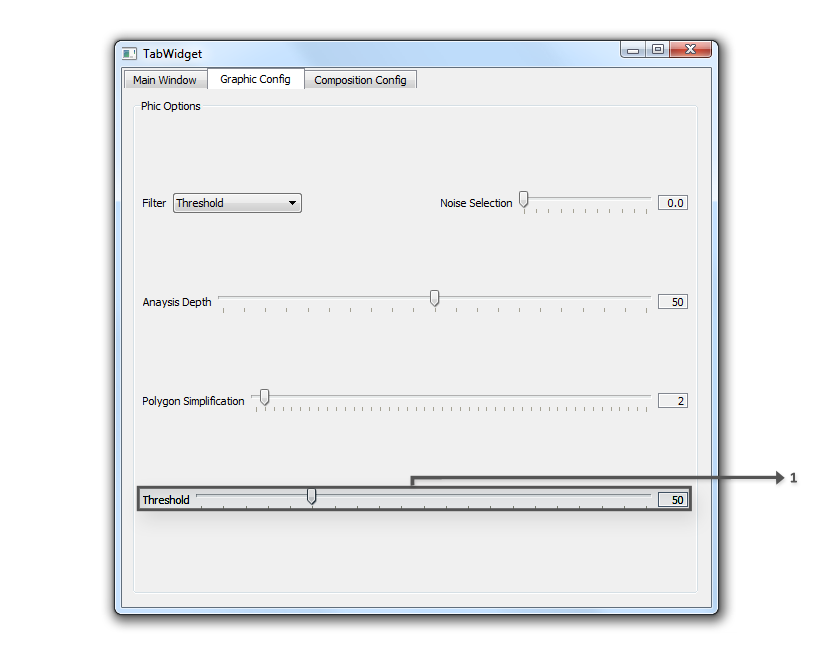
\includegraphics[scale=0.57]{graphics/interfazthreshold.png}
		\caption{Vista del filtro Threshold}
		\label{fig:interfazthreshold}
		\end{figure}
		
		Este filtro transforma la imagen a escala de grises para luego marcar como blancos todos los píxeles con un valor de gris superiores a un umbral dado, y como negros el resto.\\
		
		Los parámetros específicos que usa, vistos en la Figura~\ref{fig:interfazthreshold}, son:\\		
		
		\noindent\textit{Valor del umbral [1]:} Establece el valor del umbral antes explicado.\\
		
	\noindent\textbf{Adaptative Threshold}\\

		Mientras que el filtro anterior utiliza un mismo umbral para toda la imagen, Adaptative Threshold analiza cada parte de la imagen en escala de grises y decide qué umbral es mejor para cada sección.\\ 
		
		Este filtro no usa parámetros específicos, ya que recalcula el valor del umbral cada vez que le resulta necesario.\\
		
	\noindent\textbf{Canny}\\

		Utiliza el algoritmo de detección de regiones del mismo nombre, desarrollado en 1986 por John F. Canny. Una vez encontrados los bordes, establece las figuras que estos delimitan.\\
		
		Este filtro no usa parámetros específicos.\\
		
	\noindent\textbf{Hue Division}\\

		\begin{figure}[htbp]
		\centering
		\hspace*{-0.9in}
		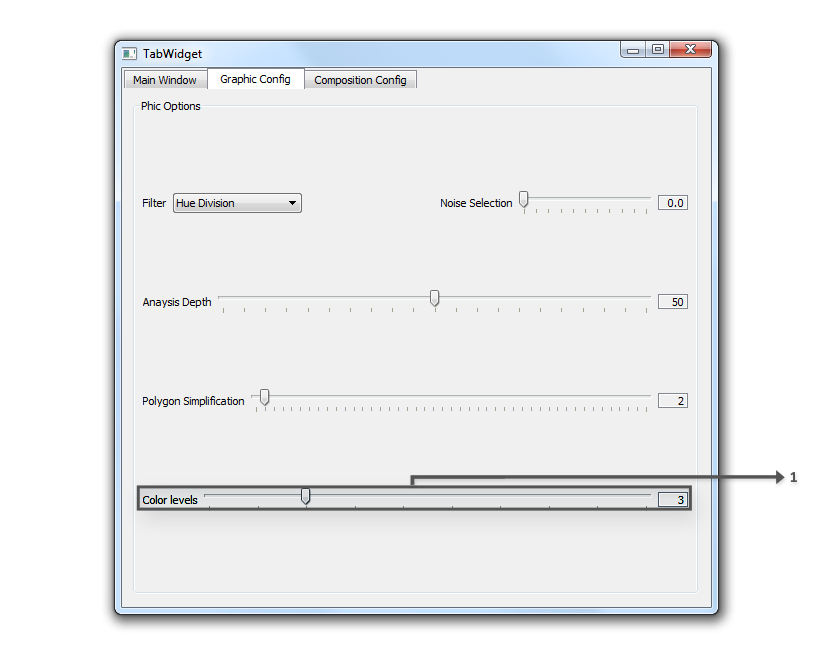
\includegraphics[scale=0.57]{graphics/interfazhue.png}
		\caption{Vista general del filtro Hue Division}
		\label{fig:interfazhue}
		\end{figure}

		Se trata de un filtro propio que busca asocia manchas de color con conjuntos de píxeles vecinos con valores RGB dentro de un mismo rango de rojo (R), azul (B) y verde (G). Los parámetros específicos son:\\
		
		\noindent\textit{Niveles de color[1]:} Este parámetro determina el número de intervalos posibles de color que puede haber en cada canal de color, y por tanto determinará la amplitud de cada rango. Un valor igual a 3 indica que un pixel cualquiera puede entrar dentro de 3 intervalos posibles en el canal rojo, otros 3 en el azul y otros 3 en el verde. De esta forma cada píxel entra dentro de una de las $3*3*3=27$ categorías de color, simplificando el análisis. Un valor muy grande de este parámetro hará que haya más categorías de color y que por tanto colores que antes se consideraban parte de una misma forma ahora se consideren como parte de formas independientes con colores más específicos. Un valor muy pequeño hará que se interpreten formas más amplias (incluyendo píxeles más diversos).\\
		
	\noindent\textbf{Color Threshold}\\

		\begin{figure}[htbp]
		\centering
		\hspace*{-0.9in}
		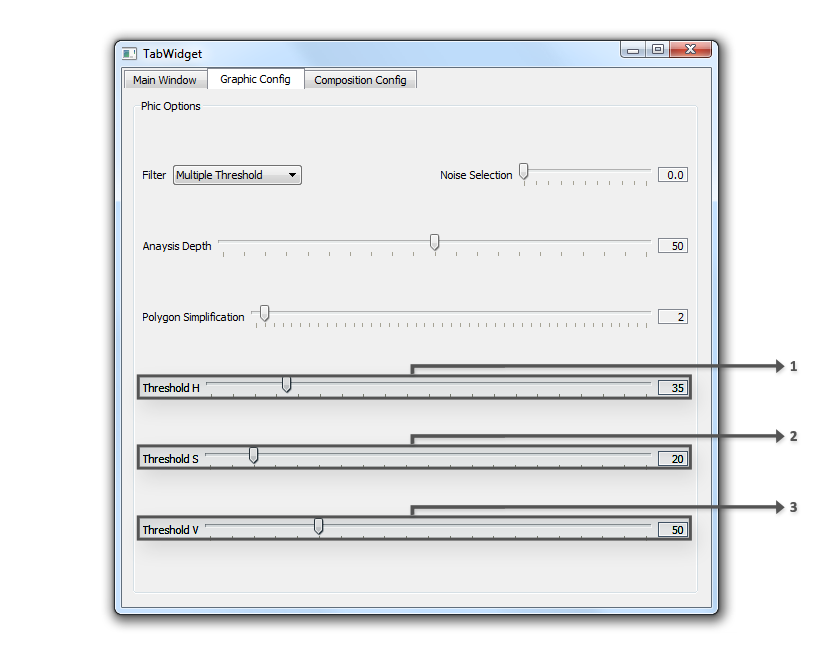
\includegraphics[scale=0.57]{graphics/interfaz3threshold.png}
		\caption{Vista general del filtro Color Threshold}
		\label{fig:interfaz3threshold}
		\end{figure}

		Se trata de un filtro propio que adapta el filtro Threshold para una imagen de 3 canales. En vez de considerar como figuras aquellas agrupaciones de píxeles cuyos valores en escala de grises sean inferiores a un umbral, considera aquellas que en su canal de Matiz (Hue), Saturación (Saturation) y Valor (Value) sean menor que un umbral, originando cada canal formas independientes.\\
		
		Los parámetros específicos de este filtro determinarán el valor de los umbrales de cada canal determinado en formato de imagen HSV.\\		
		
		\noindent\textit{Valor del umbral de Matiz[1]}\\
		\noindent\textit{Valor del umbral de Saturación[2]}\\
		\noindent\textit{Valor del umbral de Valor[3]}




		
		\subsubsection{Configuración de composición}
		
		Esta pestaña contiene todos los parámetros configurables relativos a la composición algoritmica. Estos, como muestra la Figura~\ref{fig:interfazcomp} son:\\
		
		\begin{figure}[htbp]
		\centering
		\hspace*{-0.9in}
		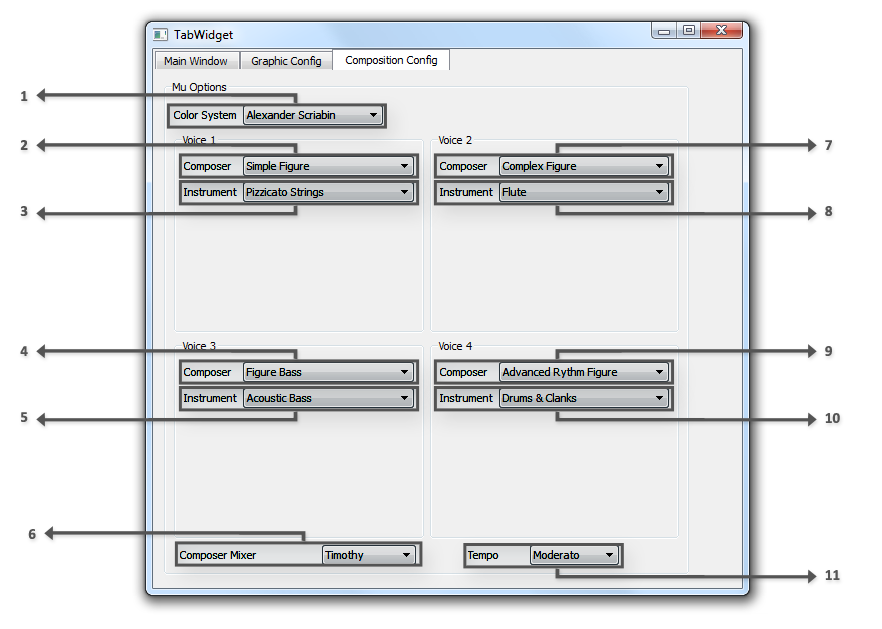
\includegraphics[scale=0.57]{graphics/interfazcomp.png}
		\caption{Vista general de la pestaña de configuración gráfica}
		\label{fig:interfazcomp}
		\end{figure}
		
		\noindent\textit{Sistema de color[1]:} Permite alternar entre las diferentes relaciones tono-color explicadas en el Capítulo~\ref{sec:algcomp}.\\
		
		\noindent\textit{Algoritmo de composición para la primera voz[2]:} Con esta opción, el usuario puede elegir, de entre los distintos algoritmos de composición, el que se usará para que generar la melodía principal.\\
		
		\noindent\textit{Algoritmo de composición para la segunda voz[7]:} Con esta opción, el usuario puede elegir, de entre los distintos algoritmos de composición, el que se usará para que generar la segunda melodía principal.\\

		\noindent\textit{Algoritmo de composición para la tercera voz[4]:} Con esta opción, el usuario puede elegir, de entre los distintos algoritmos de composición del bajo, el que se usará para que generar el bajo armónico.\\
		
		\noindent\textit{Algoritmo de composición para la cuarta voz[9]:} Con esta opción, el usuario puede elegir, de entre los distintos algoritmos de composición de ritmos, el que se usará para que generar el ritmo de la pieza musical final.\\
		
		\noindent\textit{Selección de instrumentos [3], [5], [8] y [10]:} Permiten seleccionar los instrumentos con los que sonaran las distintas voces.\\

		\noindent\textit{Algoritmo de composición general[6]:} Determina qué algoritmo se usará para recorrer la imagen y aplicar los algoritmos de las distintas voces. Se explica con detalle en el Capítulo~\ref{sec:algcomp}.\\

		\noindent\textit{Tempo[11]:} Como su nombre indica, su valor determina el tempo con el que sonará la pieza musical compuesta.\\
		
		
\section{Requisitos}
\todo{Ampliar, desarrollar, repasar y juntar las que sean redundantes o juntables (valgama la reredundancia)}
Los usuarios con los que trabajaremos para delimitar los requisitos son:
\begin{itemize}
	\item Usuario: Personas con un conocimiento mínimo o nulo sobré música y ofimática que hayan leído o se les haya explicado el funcionamiento de la aplicación
	\item Desarrollador: Personas con un conocimiento amplio de programación y con conocimiento básico o avanzado de música.
\end{itemize}
Los requisitos funcionales del proyecto son:
\\Para la interfáz gráfica:
 \begin{itemize}
	 \item La interfaz deberá ser capaz de interpretar archivos de imagen del formato .png y mostrarlos por pantalla
	 \item La interfaz deberá ser capaz de interpretar archivos de audio del formato .wav y permitir funciones básicas de reproducción sobre los mismos
	 \item La interfaz deberá ser capaz de generar un archivo de configuración interpretable por tanto Mu como Phic a partir de los parametros de entrada establecidos por el usuario.
	 \item La interfaz deberá de ser capaz de, mediante una llamada a otro programa, mostrar la partitura de la música compuesta trás haber sido generada.
	 \item La interfaz deberá controlar posibles errores cometidos por el usuario por tocar parámetros no disponibles para la configuración seleccionada, a su vez deberá de limitar las acciones del usuarilo a la hora de modificár dichos parámetros según las configuraciones elejidas.
 \end{itemize}
 Para Phy:
 \begin{itemize}
	\item El analizador deberá recibir un archivo de configuración que determine como realizar el análisis y un archivo de imagen que analizar
	\item El analizador deberá generar un archivo XML con los siguientes datos:
	\begin{itemize}
		\item Los vértices de las figuras que componen la imagen de entrada y el número total de vértices por figura.
		\item Los  colores que contienen dichas figuras en formato RGB
		\item Las figuras estarán organizadas jerárquicamente al igual que se presentan en la imagen, es decir, si una figura está dentro de otra en el XML se verá reflejado siendo la segunda figura un elemento incluido en la primera.
	\end{itemize}
	\item El analizador deberá de devolver una imagén con la representación poligonal de la imagen de entrada.
 \end{itemize}
 Para Mu:
 \begin{itemize}
	\item El compositor deberá de recibir un archivo de configuración y un archivo con los resultados del análisis correctamente estructurados.
	\item El compositor deberá generar un archivo abc interpretable por cualquier programa que pueda recibir como entrada dicho tipo de archivos.
	\item El compositor debera de ser capaz de llamar a terceros que transformen el archivo abc generado a los formatos midi y wav.
 \end{itemize}
Requisitos no funcionales:
\\Generales o/y GUI:
\begin{itemize}
	\item La aplicación facilitará al usuario la entrada de datos de configuración o imágenes que desee analizar.
	\item La aplicación facilitará al usuario los resultados del análisis hecho de la imagén de entrada.
	\item La aplicación producirá archivos de audio como resultados de la composición reproducibles en cualquier sistema con soporte básico de audio.
	\item La aplicación facilitará la reproducción de estos archivos al usuario con un reproductor de música incrustado.
	\item La aplicación facilitará el establecimiento del directorio destino de los archivos de audio.
	\item La aplicación facilitará la partitura compuesta por ella misma tras haberse generádo la música.
\end{itemize}
Phic:
\begin{itemize}
	\item Al menos uno de los analizadores devolverá un análisis que se asemeje a ''primera vista'' a la imagen original
\end{itemize}
Mu:
\begin{itemize}
	\item El compositor mediante su estructura interna facilitará al desarrollador la creación de nuevos algoritmos de composición.
	\item El compositor principal de la aplicación deberá de ser capaz de generar una música que no tenga porque ser ''interesante'' pero que ''no sonará mal'' en ambos casos los resultados en ultima instancia dependerán de la opinión subjetiva del usuario
\end{itemize}
\todo{TENEMOS QUE HABLAR DE ESTO Y COSAS}

	usuarios\\
	\begin{itemize}
		\item usuario casual
		\item usuario avanzado
		\item desarrollador?\\
	\end{itemize}

	requisitos\\
	\begin{itemize}
		\item analizar imagenes a un formato directo de composicion
		componer analisis
		\item permitir variar parametros de analisis
		\item permitir variar parametros de composicion
		\item multiplataforma\\
	\end{itemize}
		
		
	restricciones\\
	\begin{itemize}
		\item el sistema debe ser lo suficientemente flexible como para permitir expandirse con otros lenguajes
		\item el analisis y composicion no deben consumir muchos recursos\\
	\end{itemize}
		
	requisitos no funcionales (nombrados en la intro)\\
	\begin{itemize}	
		\item No se tienen en cuenta objetos físicos en el analisis, solo color
		\item El único componente de entrada usado es la imagen dada, nada de musica externa ya creada.
		\item Generación de contenido frente a acoplamiento de creaciones preestablecidas	\\	
	\end{itemize}		
		
		
Casos de uso?

	(analisis: explicar proceso de filtrado y en sistema explicar solo la arquitectura de clases?)
\section{Arquitectura}

\subsection{Formato de representación de música}

\todo{Repasar formalizar}

La estructura para representar la música propuesta en el proyecto está determinada por un árbol que trabaja desde el elemento más general, la canción que se va a componer, al más específico, cada una de las notas que componen dicha canción, como muestra la Figura~\ref{fig:structmusic}.\\
	
	\begin{figure}[htbp]
	\centering
	\hspace*{-0.67in}
	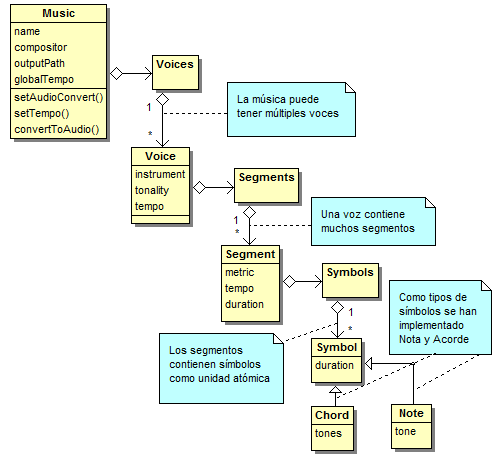
\includegraphics[scale=0.57]{graphics/musica-estructura.png}
	\caption{Estructura de la música}
	\label{fig:structmusic}
	\end{figure}


\textbf{Música}: Al nivel de la Música, trabajamos con la información relativa a toda la canción que se va a componer, por un lado está información relativa al nombre de la composición y del compositor que la ha hecho, también dispone de una serie de voces a partir de las cuales estará formada la canción y su tempo. Por último a un nivel más cercano, la implementación permitirá elegir con que herramienta querremos crear el archivo de audio de salida.
\newline

\textbf{Voz}: Por debajo de la Música se trabaja con las Voces. Su estructura permite determinar el instrumento, la tonalidad y el tempo de cada una de las voces que componen una Música, cada una de estas voces esta compuesta de varios segmentos musicales, los cuales al ser reproducidos en el orden establecido por el compositor forman la Voz en cuestión.
\newline

\textbf{Segmento}: Estos elementos tienen la posibilidad de establecer su propia métrica, su tempo y su duración. Los segmentos a su vez están formados por una sucesión de símbolos.
\newline

\textbf{Símbolo}: Son la unidad a partir de los cuales se crean todos los elementos básicos de la música, símbolo nos permite establecer una duración para estos elementos. Actualmente el proyecto crea dos tipos de elementos a partir de símbolo:
\begin{itemize}
\item \textbf{Notas}: Estos símbolos tienen asociada una duración, determinada por el componente anterior, y un tono establecido por un número que posteriormente será interpretado con la herramienta que generará el archivo de audio.
\item \textbf{Acordes}: Los acordes están formados de la misma manera que las notas pero en lugar de tener asociado un único tono pueden tener de dos a tres tonos diferentes, en la práctica esto resultará en todos los tonos sonando a la vez durante el mismo tiempo una vez generada la canción.
\end{itemize}

\subsection{Formato de representación de imágenes}

\todo{está en google docs, sólo es pasarlo a limpio}

\subsection{Sistema de análisis de Imágenes: Phic}

\todo{hacer}

\subsection{Sistema de composición algorítmica: Mu}

\todo{hacer}

\subsection{Sistema de enlace de módulos: Muphic}

\todo{hacer}

\subsubsection{Interfaz Gráfica}

El desarrollo de la interfáz gráfica se decidió realizar a través de un framework que facilitase la construcción de la misma. Qt, la herramienta que se utilizó se eligió debido a dos criterios, era multiplataforma, al igual que la aplicación, servía para trabajar con móviles, siguiendo así uno de los enfoques iniciales del proyecto que más adelante fue descartado. Además Qt trabaja con C++ como lenguaje de programación, el mismo que el núcleo de la aplicación y ofrece facilidades a la hora de integrar audio, a través de la librería Phonon, o componentes personalizados en una interfaz.\\
\todo{Este párrafo no se si abriría mejor la parte de arquitectura}
\newline
La interfáz esta compuesta de tres pestañas cada una encargada de una parte de la funcionalidad:
\newline
\\\underline{Graphic Config:}
\\En esta pestaña se encuentran todas las opciones relacionadas con el análisis de la imagen, las distintas configuraciones se transmitirán a los módulos de la aplicación a través de un documento XML que se genera cuando en la "Main Window" se le da al boton de "Analyze".
\\Los distintos componentes de esta pestaña van variando según el filtro que se seleccione, sin embargo algunos de ellos son comunes para todos los filtros:
\newline
\\\textit{Filter:} Este combo box permite seleccionar entre los distintos filtros que se pueden usar en la aplicación.
\\\textit{Noise Selection:} Con esta barra de desplazamiento se podrá elegir a partir de que tamaño, relativo al area del mayor polígono de la imagen, se ignorarán los poligonos encontrados durante el análisis de la imagen.
\\\textit{Analysis Depth:} Esta barra permite seleccionar cuanto deseamos comprimir la imagen original antes de analizarla, cuando menor sea su valor menor será el nivel de detalle obtenido y más rápido se realizará el análisis.
\\\textit{Polygon Simplification:} Esta barra permite seleccionar cuanto deseamos simplificar los poligonos obtenidos a partir de la imagen original, cuanto mayor sea su valor menos vertices tendrán los poligonos obtenidos y por lo tanto menos fiel será el resultado del análisis, sin embargo, este se realizará más rápido.
\newline
\\Según el filtro que se elija aparecerán mas componentes:
\newline
\\\todo{Rellenar esto de manera experta y didáctica}
\\\textit{Threshold} (Filtro Threshold): 
\\\textit{Hue Division} (Filtro Hue Division):
\\\textit{Threshold H} (Filtro Multiple Threshold):
\\\textit{Threshold S} (Filtro Multiple Threshold):
\\\textit{Threshold V} (Filtro Multiple Threshold):
\newline
\\\underline{Composition Config:}
\\En esta pestaña se pueden encontrar todas las opciones disponibles para el compositor musical, estás serán transmitidas a los modulos de la aplicacióncuando se pulse el boton de "Compose" en la "Main Window" a través del documento XML mencionado anteriormente.
\\Como se puede ver en la imagen adjunta, hay opciones para cuatro voces, que son aquellas con las que trabajan los compositores de la aplicación siendo, normalmente, la "Voice 1" la melodía principal, la "Voice 2" un acompañamiento, la "Voice 3" el bajo y la "Voice 4" la percusión. Las opciones disponibles son las siguientes:
\\\todo{Adjuntar imagen}
\newline
\\textit{Color System:} Hace referencia referencia a la teoría sinestésica que se utilizará como base para la relación de color-notas durante la composición musical.
\\textit{Composer:} En las cuatro voces se refiere a que compositor se utilizará para esa voz, al presionarlo se desplegarán los distintos compositores que estan disponibles para que el usuario elija el que mejor le convenga.
\\textit{Instrument:} En las cuatro voces se refiere a que instrumento se utilizará para esa voz en concreto, al presionarlo se desplegarán los instrumentos disponibles.
\\textit {Composer Mixer:} Hace referencia a que como se combinarán las cuatro voces anteriores.
\\textit{Tempo:} 
\\\todo{A rellenar con gente que sepa describirlo mejor que yo. \\También hay que repasar lo anterior}
\newline
\\{\bf Libreria Phonon}
\\Esta es una librería proporcionada por Qt para la reproducción de audio, al ser un módulo externo requiere una serie de librerias añadidas que están incluidas en el paquete de instalación de windows, sin embargo tendrán que ser instaladas en linux utilizando alguno de los gestores de software disponibles realizando una busqueda con la palabra clave: Phonon.
\\Las librerías requeridas son las siguientes: (LISTA DE LIBRERIAS)
\\En el caso de que no funcione el sistema de reproducción, se pueden encontrar los archivos de audio en la ruta especificada en "Midi Output"
\newline
\\\todo{Claramente esta parte va en arquitectura, sin embargo no se que más comentar de la arquitectura de la GUI puesto que casi todo esta hecho con QT, como no digamos el widget de carlos...}
\\La interacción con phonon se realiza utilizando la funcionalidad proporcionada por el framework. Se asocia el fichero multimedia a un tipo proporcionado por Phonon que a su vez lo conecta con el sistema de audio predeterminado para cada sistema operativo.
\\El uso de Phonon es conveniente porque a pesar de sus complicaciones ofrece una manera sencilla de incluir un reproductor en la interfaz, que a su vez, es multiplataforma sin obligar al usuario a buscar el archivo de audio o forzar una llamada a un tercer programa que reproducir la musica que generada.
\subsection{Futuras ampliaciones}